\documentclass[review,sigconf]{acmart}

\usepackage{graphicx}
\usepackage{listings}
\usepackage{multirow}
\usepackage{balance}
\usepackage{amsmath}
\usepackage{framed}
\usepackage{subfigure}

\newcommand{\todo}[1]{\textcolor{red}{TODO: #1}}

\begin{document}

\title[omr-lilypond-midi]{Optical Music Recognition for LilyPond File Generation}
\author{Evan Matthews}
\email{evanmm3@illinois.edu}
%\orcid{1234-5678-9012}
\affiliation{%
	\institution{University of Illinois Urbana-Champaign}
	\country{}
}

\begin{abstract}
\todo{Abstract}
\end{abstract}

\maketitle

\section{Introduction}
\todo{Introduction}
\cite{oord2016wavenet,contreras2023omrcnn,contreras2023omrpiano,mayer2024practical,andrea2021note}

In the world of music or audio transcription/arrangement, the complexity of sound and score data has allowed human performance to remain the current state-of-the-art. Several factors contribute to this circumstance: the number of potential audio and score file types, ambiguity on how performance qualities are notated, and overall inconsistencies between recordings and their respective scores. Machine learning models, in turn, have been a crucial step towards reducing these inconsistencies. Their ability to learn the nonlinearities and artistic qualities that otherwise plague audio computation have allowed for noteworthy advancements such as the WaveNet~\cite{oord2016wavenet}. The remaining issue in the process of sound generation is the amount of data available to train with. Worthwhile audio data remains difficult to collect due to its large size and potential copyright issues. In particular, trying to condition off another medium is incredibly difficult as current datasets lack the correlations necessary to streamline the audio transcription process. Datasets such as MAESTRO are close to ideal results, but some intermediate steps are needed to learn correlations between audio files and musical scores.

With the following conditions in mind, I propose an Image-to-MIDI model to serve a few purposes. First, this model serves to convert image data to relative musical data to a high degree of accuracy. The process of converting MIDI to an image is trivial, but the opposite is a known Optical Music Recognition (OMR) problem in that the correlation is nonexistent. 
Second, a highly reliable model of this type is capable of serving as an intermediate step in future audio computation endeavors, as the nontrivial nature of OMR is a barrier for reliable model training between scores and other types of audio data. 
Finally, a conversion of this type allows for more flexible datasets because MIDI can be converted into a number of other audio file types.

This model generally references existing OMR research and serves as an attempt to construct a completely new CNN model. Existing MIDI datasets have been narrowed down to strictly two-stave piano works by Johann Sebastian Bach to maintain rhythmic and compositional uniformity, although a generalized model for various instruments and number of staves can theoretically be produced given a large enough dataset.


\section{Background}
\subsection{Optical Music Recognition}
\todo{OMR background}

\subsection{Lilypond}
Lilypond was chosen for dataset file representation as it maintains accurate translation between digital (MIDI) and visual (image) notation systems~\cite{lilypond}.
In particular, translation from Lilypond to MIDI is trivial, and Lilypond provides a more intuitive representation of musical information compared to raw bytes of MIDI data.
This notation language consists of multiple layers to separate score components:

\begin{itemize}
		\item \textbf{Document level:} components related to page layout and high-level musical details, (number of instruments/tracks, score engraving information).
		\item \textbf{Music level:} components related to low-level musical details, (notes, rhythms, durations, key/time signatures, tempo).
\end{itemize}

At the document level, \todo{document}

\begin{figure*}
	\begin{subfigure}
		\centering
		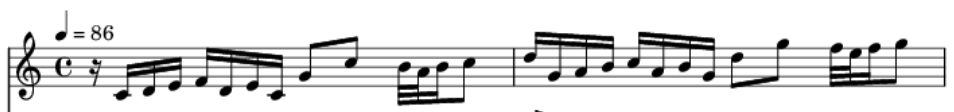
\includegraphics[width = .8\linewidth]{./figures/lilypond-snippet.png}
		% \caption{Rendered Lilypond (.ily) file with code}
		\label{fig:lilypond-snippet}
	\end{subfigure}
	~
	\begin{subfigure}
		\centering
		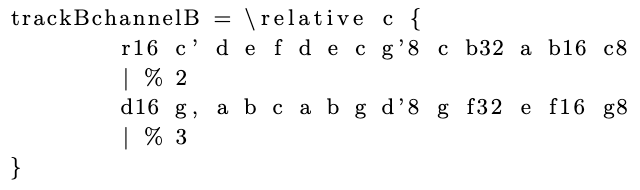
\includegraphics[width = .8\linewidth]{./figures/lilypond-code.png}
		\label{fig:lilypond-code}
	\end{subfigure}
	\caption{Lilypond (.ily) code and rendering, (time signature = 4/4)}
	\label{fig:lilypond-example}
\end{figure*}

At the music level, rhythmic musical symbols are notated according to their pitches and relative time duration.
pitches are all characters ${a, b, c, d, e, f, g, r}$, where $r$ is a "rest" meaning no pitch occurs.
To ascend or descend in pitch beyond a single musical "octave," the $'$ and $,$ characters are appended to indicate one or more octave ascendings or descendings, respectively.
Pitches are also proceeded by a rhythmic value representing its duration in time.
These values are typically powers of two, (but can technically be any positive floating-point value), and they dictate how long a pitch is played with respect to the piece's time signature.
For example, a score with time signature = 2/4 indicates that each measure has two beats, and each beat is the length of a quarter note (hard-coded in the denominator).
In this case, the line $"c4 d4"$ would represent two quarter (4) notes or a single measure in the provided time signature.
Additionally, notes without defined durational values take on the previous note's duration in a line, so a series of equal-duration notes is represented by one durational value.
Finally, separations between measures are made with $"| \% n"$, marking the end of measure $n$.
Figure~\ref{fig:lilypond-example} compares the rendering of a single staff of music with its relative Lilypond notation .

% \begin{lstlisting}
% trackBchannelB = \relative c {
% 	r16 c' d e f d e c g'8 c b32 a b16 c8 
% 	| % 2
% 	d16 g, a b c a b g d'8 g f32 e f16 g8 
% 	| % 3
% }
% \end{lstlisting}


\section{Experiment}
\subsection{Key resources}
\todo{Remove this section?}
The Image-to-MIDI convolutional neural network will be built from scratch while referencing promising results from OMR and image-to-text research, (should the CNN need fine-tuning or other enhancement). Currently, the model dataset is the complete Bach Midi Index and will be narrowed down to fit additional constraints: two staves, single instrument, rhythmic quantization at the 16th or 32nd- note level. Model testing will focus primarily on self-trained work, but I am interested in comparing against pre-trained models if I have extra time. For hardware, training will take place on a Linux GPU cluster, courtesy of Paris Smaragdis and the UIUC-CS Audio Computing Lab. Programming work is using a combination of Python with Pytorch for the CNN, and Bash scripts with Lilypond to prepare and normalize the dataset.

\subsection{Dynamic quantization}
\todo{quantization stuff}

\subsection{CRNN Model}
\todo{CRNN model}

\section{Results}

\section{Discussion}
\todo{discussion}

\section{Conclusions}
\todo{conclusions}

\bibliographystyle{ACM-Reference-Format}
\bibliography{references-cs444}

\end{document}